\documentclass[14pt]{extbook}
\usepackage{multicol, enumerate, enumitem, hyperref, color, soul, setspace, parskip, fancyhdr} %General Packages
\usepackage{amssymb, amsthm, amsmath, bbm, latexsym, units, mathtools} %Math Packages
\everymath{\displaystyle} %All math in Display Style
% Packages with additional options
\usepackage[headsep=0.5cm,headheight=12pt, left=1 in,right= 1 in,top= 1 in,bottom= 1 in]{geometry}
\usepackage[usenames,dvipsnames]{xcolor}
\usepackage{dashrule}  % Package to use the command below to create lines between items
\newcommand{\litem}[1]{\item#1\hspace*{-1cm}\rule{\textwidth}{0.4pt}}
\pagestyle{fancy}
\lhead{Progress Quiz 4}
\chead{}
\rhead{Version B}
\lfoot{6286-1986}
\cfoot{}
\rfoot{Fall 2020}
\begin{document}

\begin{enumerate}
\litem{
Factor the quadratic below. Then, choose the intervals that contain the constants in the form $(ax+b)(cx+d); b \leq d.$\[ 36x^{2} +11 x -12 \]\begin{enumerate}[label=\Alph*.]
\item \( a \in [0, 2.8], \hspace*{5mm} b \in [-21, -10], \hspace*{5mm} c \in [-0.42, 1.09], \text{ and } \hspace*{5mm} d \in [25, 32] \)
\item \( a \in [16.2, 21.8], \hspace*{5mm} b \in [-7, 0], \hspace*{5mm} c \in [1.93, 2.39], \text{ and } \hspace*{5mm} d \in [1, 5] \)
\item \( a \in [1.1, 4.3], \hspace*{5mm} b \in [-7, 0], \hspace*{5mm} c \in [10.71, 13.46], \text{ and } \hspace*{5mm} d \in [1, 5] \)
\item \( a \in [8.4, 12.7], \hspace*{5mm} b \in [-7, 0], \hspace*{5mm} c \in [3.15, 5.03], \text{ and } \hspace*{5mm} d \in [1, 5] \)
\item \( \text{None of the above.} \)

\end{enumerate} }
\litem{
Solve the quadratic equation below. Then, choose the intervals that the solutions belong to, with $x_1 \leq x_2$ (if they exist).\[ 18x^{2} -8 x -7 = 0 \]\begin{enumerate}[label=\Alph*.]
\item \( x_1 \in [-0.94, -0.8] \text{ and } x_2 \in [0, 0.5] \)
\item \( x_1 \in [-8.21, -7.8] \text{ and } x_2 \in [14.6, 16.5] \)
\item \( x_1 \in [-24.14, -23.48] \text{ and } x_2 \in [21.9, 26.5] \)
\item \( x_1 \in [-0.57, -0.05] \text{ and } x_2 \in [0.8, 1.6] \)
\item \( \text{There are no Real solutions.} \)

\end{enumerate} }
\litem{
Write the equation of the graph presented below in the form $f(x)=ax^2+bx+c$, assuming  $a=1$ or $a=-1$. Then, choose the intervals that $a, b,$ and $c$ belong to.
\begin{center}
    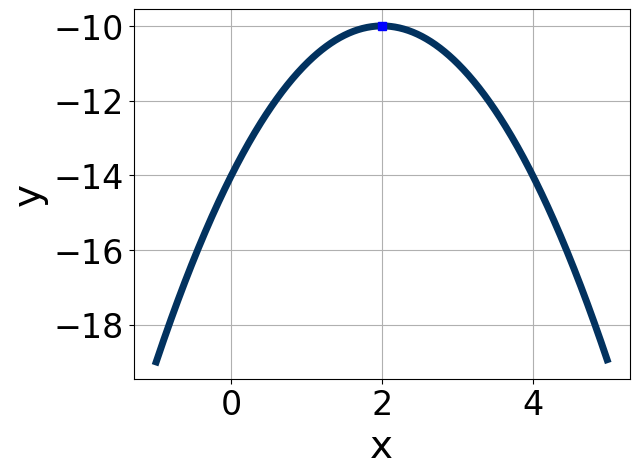
\includegraphics[width=0.5\textwidth]{../Figures/quadraticGraphToEquationB.png}
\end{center}
\begin{enumerate}[label=\Alph*.]
\item \( a \in [-2.2, -0.8], \hspace*{5mm} b \in [-5, 0], \text{ and } \hspace*{5mm} c \in [4, 8] \)
\item \( a \in [-0.3, 1.4], \hspace*{5mm} b \in [3, 5], \text{ and } \hspace*{5mm} c \in [-8, -3] \)
\item \( a \in [-0.3, 1.4], \hspace*{5mm} b \in [-5, 0], \text{ and } \hspace*{5mm} c \in [-8, -3] \)
\item \( a \in [-2.2, -0.8], \hspace*{5mm} b \in [-5, 0], \text{ and } \hspace*{5mm} c \in [-15, -13] \)
\item \( a \in [-2.2, -0.8], \hspace*{5mm} b \in [3, 5], \text{ and } \hspace*{5mm} c \in [-15, -13] \)

\end{enumerate} }
\litem{
Graph the equation below.\[ f(x) = (x+2)^2 - 10 \]\begin{enumerate}[label=\Alph*.]
\begin{multicols}{2}\item 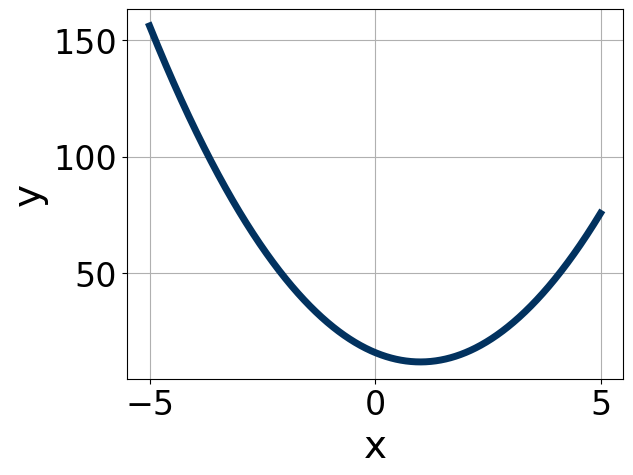
\includegraphics[width = 0.3\textwidth]{../Figures/quadraticEquationToGraphAB.png}\item 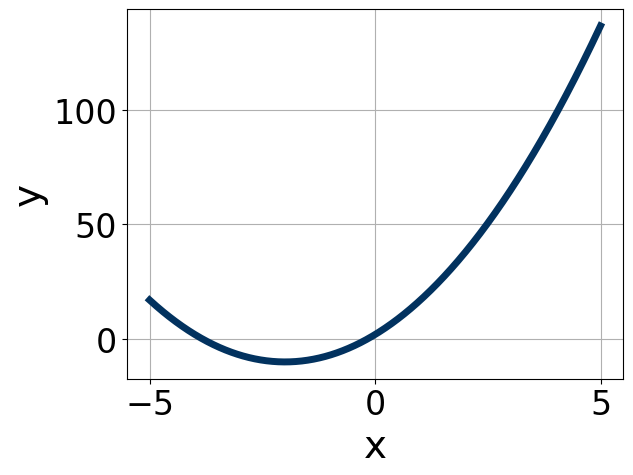
\includegraphics[width = 0.3\textwidth]{../Figures/quadraticEquationToGraphBB.png}\item 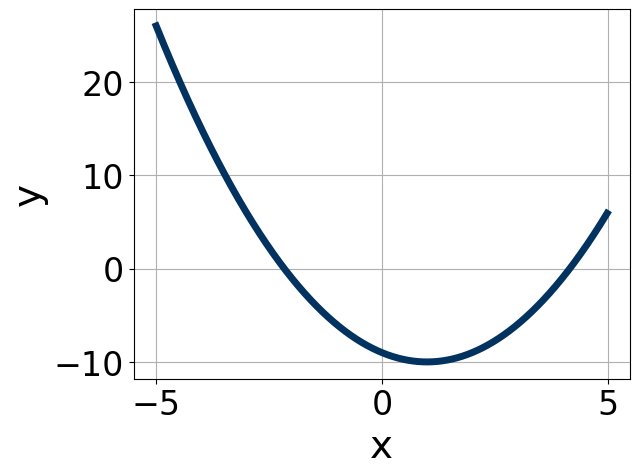
\includegraphics[width = 0.3\textwidth]{../Figures/quadraticEquationToGraphCB.png}\item 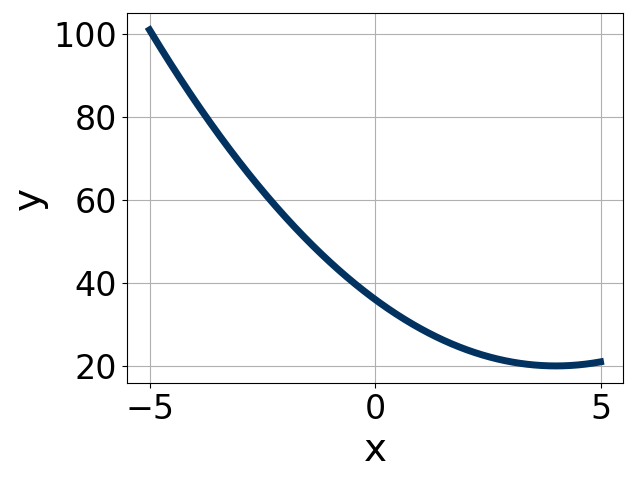
\includegraphics[width = 0.3\textwidth]{../Figures/quadraticEquationToGraphDB.png}\end{multicols}\item None of the above.
\end{enumerate} }
\litem{
Write the equation of the graph presented below in the form $f(x)=ax^2+bx+c$, assuming  $a=1$ or $a=-1$. Then, choose the intervals that $a, b,$ and $c$ belong to.
\begin{center}
    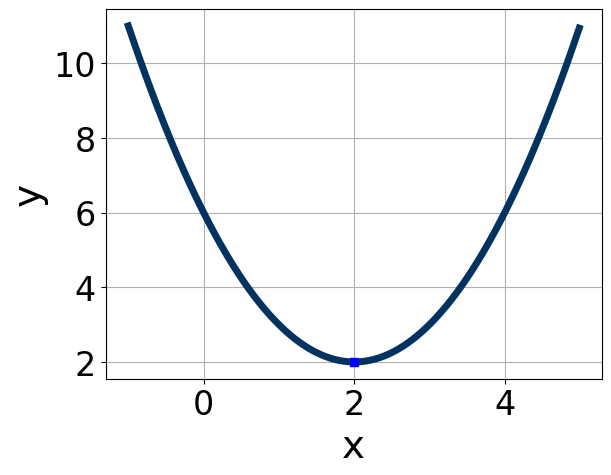
\includegraphics[width=0.5\textwidth]{../Figures/quadraticGraphToEquationCopyB.png}
\end{center}
\begin{enumerate}[label=\Alph*.]
\item \( a \in [-0.7, 1.3], \hspace*{5mm} b \in [-6, 0], \text{ and } \hspace*{5mm} c \in [5, 9] \)
\item \( a \in [-3.1, 0.8], \hspace*{5mm} b \in [4, 6], \text{ and } \hspace*{5mm} c \in [-7, 0] \)
\item \( a \in [-0.7, 1.3], \hspace*{5mm} b \in [4, 6], \text{ and } \hspace*{5mm} c \in [2, 4] \)
\item \( a \in [-0.7, 1.3], \hspace*{5mm} b \in [4, 6], \text{ and } \hspace*{5mm} c \in [5, 9] \)
\item \( a \in [-3.1, 0.8], \hspace*{5mm} b \in [-6, 0], \text{ and } \hspace*{5mm} c \in [-7, 0] \)

\end{enumerate} }
\litem{
Graph the equation below.\[ f(x) = (x+4)^2 + 18 \]\begin{enumerate}[label=\Alph*.]
\begin{multicols}{2}\item 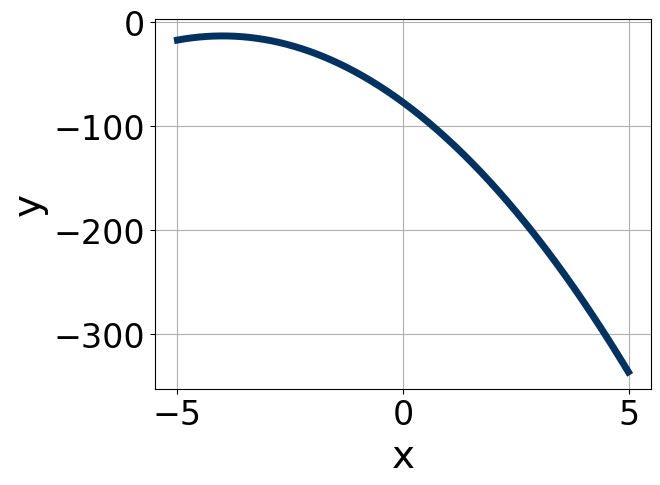
\includegraphics[width = 0.3\textwidth]{../Figures/quadraticEquationToGraphCopyAB.png}\item 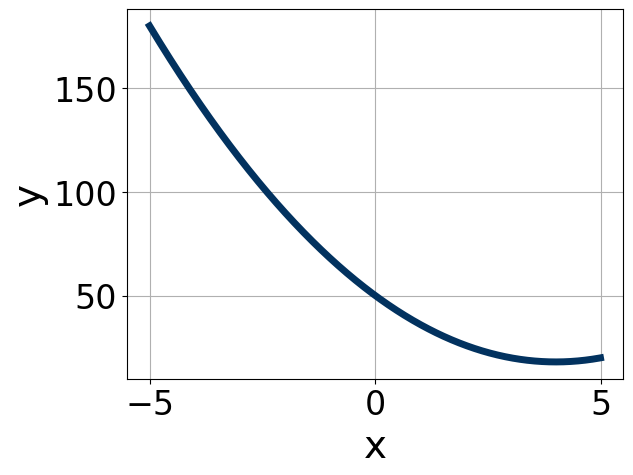
\includegraphics[width = 0.3\textwidth]{../Figures/quadraticEquationToGraphCopyBB.png}\item 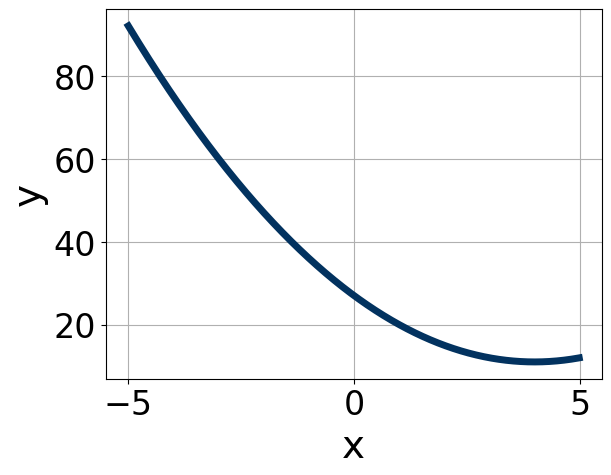
\includegraphics[width = 0.3\textwidth]{../Figures/quadraticEquationToGraphCopyCB.png}\item 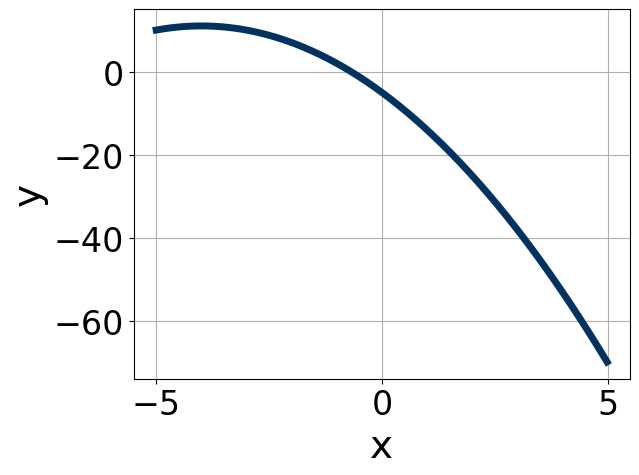
\includegraphics[width = 0.3\textwidth]{../Figures/quadraticEquationToGraphCopyDB.png}\end{multicols}\item None of the above.
\end{enumerate} }
\litem{
Factor the quadratic below. Then, choose the intervals that contain the constants in the form $(ax+b)(cx+d); b \leq d.$\[ 36x^{2} -7 x -15 \]\begin{enumerate}[label=\Alph*.]
\item \( a \in [0.44, 1.07], \hspace*{5mm} b \in [-34, -26], \hspace*{5mm} c \in [0.95, 2.15], \text{ and } \hspace*{5mm} d \in [13, 22] \)
\item \( a \in [11.92, 12.51], \hspace*{5mm} b \in [-7, 1], \hspace*{5mm} c \in [2.96, 3.08], \text{ and } \hspace*{5mm} d \in [3, 7] \)
\item \( a \in [1.89, 2.21], \hspace*{5mm} b \in [-7, 1], \hspace*{5mm} c \in [17.55, 20.08], \text{ and } \hspace*{5mm} d \in [3, 7] \)
\item \( a \in [3.97, 4.08], \hspace*{5mm} b \in [-7, 1], \hspace*{5mm} c \in [7.56, 9.39], \text{ and } \hspace*{5mm} d \in [3, 7] \)
\item \( \text{None of the above.} \)

\end{enumerate} }
\litem{
Solve the quadratic equation below. Then, choose the intervals that the solutions $x_1$ and $x_2$ belong to, with $x_1 \leq x_2$.\[ 15x^{2} -38 x + 24 = 0 \]\begin{enumerate}[label=\Alph*.]
\item \( x_1 \in [1.1, 1.28] \text{ and } x_2 \in [1.32, 1.71] \)
\item \( x_1 \in [0.43, 0.56] \text{ and } x_2 \in [3.59, 3.98] \)
\item \( x_1 \in [0.38, 0.4] \text{ and } x_2 \in [3.77, 4.04] \)
\item \( x_1 \in [0.51, 0.74] \text{ and } x_2 \in [2.28, 2.82] \)
\item \( x_1 \in [17.9, 18.03] \text{ and } x_2 \in [19.65, 20.26] \)

\end{enumerate} }
\litem{
Solve the quadratic equation below. Then, choose the intervals that the solutions belong to, with $x_1 \leq x_2$ (if they exist).\[ -18x^{2} -14 x + 7 = 0 \]\begin{enumerate}[label=\Alph*.]
\item \( x_1 \in [-1.01, -0.08] \text{ and } x_2 \in [0.5, 2.8] \)
\item \( x_1 \in [-7.03, -6.12] \text{ and } x_2 \in [19.7, 21.1] \)
\item \( x_1 \in [-27.45, -26.44] \text{ and } x_2 \in [24.9, 28.8] \)
\item \( x_1 \in [-1.79, -0.87] \text{ and } x_2 \in [-0.9, 1.1] \)
\item \( \text{There are no Real solutions.} \)

\end{enumerate} }
\litem{
Solve the quadratic equation below. Then, choose the intervals that the solutions $x_1$ and $x_2$ belong to, with $x_1 \leq x_2$.\[ 25x^{2} -10 x -24 = 0 \]\begin{enumerate}[label=\Alph*.]
\item \( x_1 \in [-20.89, -18.96] \text{ and } x_2 \in [29.23, 30.23] \)
\item \( x_1 \in [-1.17, -0.57] \text{ and } x_2 \in [1.12, 1.31] \)
\item \( x_1 \in [-5.67, -3.57] \text{ and } x_2 \in [0.21, 0.33] \)
\item \( x_1 \in [-0.76, 1.16] \text{ and } x_2 \in [2.97, 4.08] \)
\item \( x_1 \in [-3.35, -1.33] \text{ and } x_2 \in [0.29, 1.19] \)

\end{enumerate} }
\end{enumerate}

\end{document}